% 声明文件类型
\documentclass[12pt,a4paper,oneside]{ctexart}

% 声明所需要用到的宏包
\usepackage{amsmath}
\usepackage{hyperref}
\usepackage{bookmark}
\usepackage{graphicx}

% 导言区
\title{HelloTex}
\author{rootership}
\date{\today}

% 主体框架
\begin{document}
\maketitle
\tableofcontents
\section{first section}  
  \subsection{第一节}
    \paragraph{终于结束了}
\section{second section}
  \subsection{第一节}
    \paragraph{sgyhsgygsyyudghygdfyfcvbcghhefbcbshbcusxih}
    \begin{enumerate}
      \item[(1)] 第一点
      \item[(2)] 第二点
      \item[(3)] 第三点
    \end{enumerate}
\section{third section}
  \subsection{第一节}
    \paragraph{
    详情请看下图
    \begin{figure}[htbp]
      \centering
      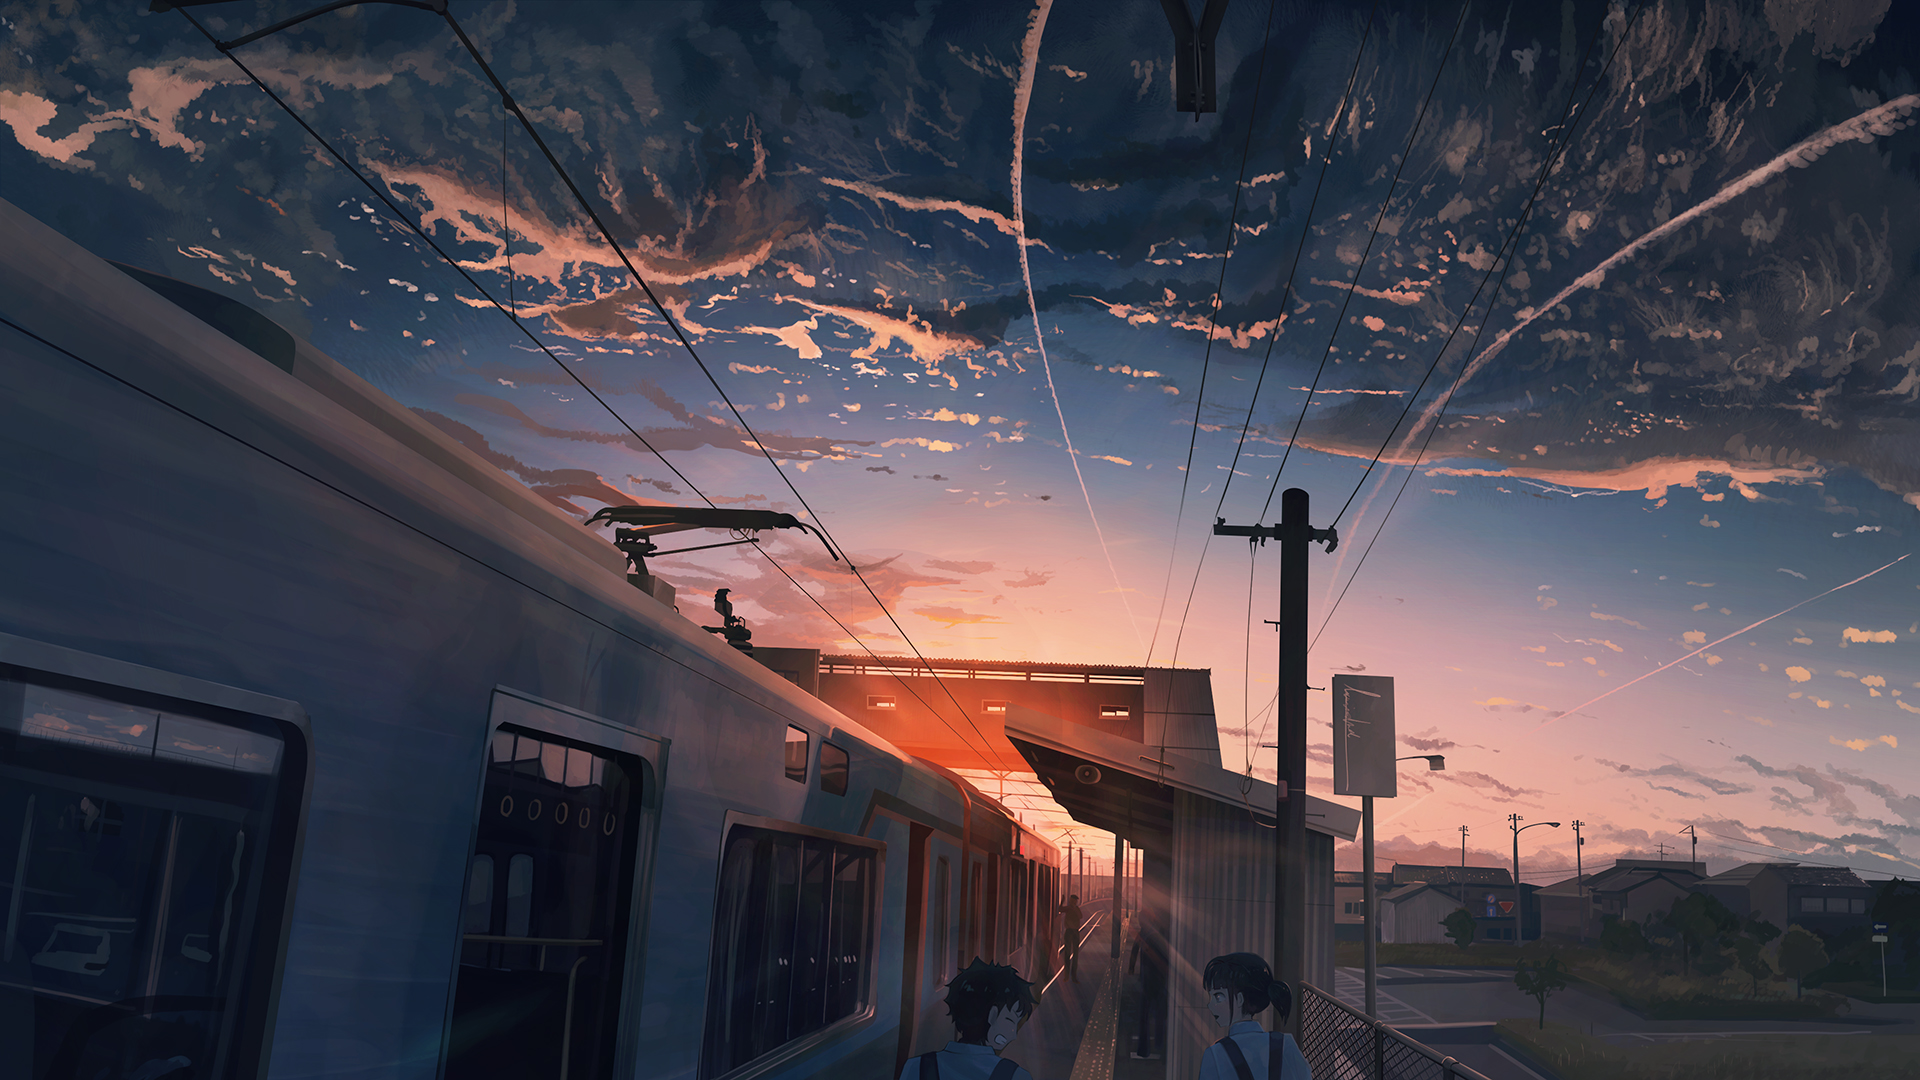
\includegraphics[width=10cm]{bg2.jpg}
      \caption{exp}
    \end{figure}
    \begin{table}[htbp]
      \centering
      \caption{fig 1}
      \begin{tabular}{lllll}
      1 & 1 & 1 & 1 & 1 \\
      1 & 1 & 1 & 1 & 1 \\
      1 & 1 & 1 & 1 & 1 \\
        &   &   &   &  
      \end{tabular}
    \end{table}
  }
  \newpage
  \section{disijie}
\end{document}